% Options for packages loaded elsewhere
\PassOptionsToPackage{unicode}{hyperref}
\PassOptionsToPackage{hyphens}{url}
%
\documentclass[
]{article}
\usepackage{amsmath,amssymb}
\usepackage{lmodern}
\usepackage{ifxetex,ifluatex}
\ifnum 0\ifxetex 1\fi\ifluatex 1\fi=0 % if pdftex
  \usepackage[T1]{fontenc}
  \usepackage[utf8]{inputenc}
  \usepackage{textcomp} % provide euro and other symbols
\else % if luatex or xetex
  \usepackage{unicode-math}
  \defaultfontfeatures{Scale=MatchLowercase}
  \defaultfontfeatures[\rmfamily]{Ligatures=TeX,Scale=1}
\fi
% Use upquote if available, for straight quotes in verbatim environments
\IfFileExists{upquote.sty}{\usepackage{upquote}}{}
\IfFileExists{microtype.sty}{% use microtype if available
  \usepackage[]{microtype}
  \UseMicrotypeSet[protrusion]{basicmath} % disable protrusion for tt fonts
}{}
\makeatletter
\@ifundefined{KOMAClassName}{% if non-KOMA class
  \IfFileExists{parskip.sty}{%
    \usepackage{parskip}
  }{% else
    \setlength{\parindent}{0pt}
    \setlength{\parskip}{6pt plus 2pt minus 1pt}}
}{% if KOMA class
  \KOMAoptions{parskip=half}}
\makeatother
\usepackage{xcolor}
\IfFileExists{xurl.sty}{\usepackage{xurl}}{} % add URL line breaks if available
\IfFileExists{bookmark.sty}{\usepackage{bookmark}}{\usepackage{hyperref}}
\hypersetup{
  pdftitle={Totota Analysis},
  pdfauthor={Sakthivel Sinnasamy},
  hidelinks,
  pdfcreator={LaTeX via pandoc}}
\urlstyle{same} % disable monospaced font for URLs
\usepackage[margin=1in]{geometry}
\usepackage{color}
\usepackage{fancyvrb}
\newcommand{\VerbBar}{|}
\newcommand{\VERB}{\Verb[commandchars=\\\{\}]}
\DefineVerbatimEnvironment{Highlighting}{Verbatim}{commandchars=\\\{\}}
% Add ',fontsize=\small' for more characters per line
\usepackage{framed}
\definecolor{shadecolor}{RGB}{248,248,248}
\newenvironment{Shaded}{\begin{snugshade}}{\end{snugshade}}
\newcommand{\AlertTok}[1]{\textcolor[rgb]{0.94,0.16,0.16}{#1}}
\newcommand{\AnnotationTok}[1]{\textcolor[rgb]{0.56,0.35,0.01}{\textbf{\textit{#1}}}}
\newcommand{\AttributeTok}[1]{\textcolor[rgb]{0.77,0.63,0.00}{#1}}
\newcommand{\BaseNTok}[1]{\textcolor[rgb]{0.00,0.00,0.81}{#1}}
\newcommand{\BuiltInTok}[1]{#1}
\newcommand{\CharTok}[1]{\textcolor[rgb]{0.31,0.60,0.02}{#1}}
\newcommand{\CommentTok}[1]{\textcolor[rgb]{0.56,0.35,0.01}{\textit{#1}}}
\newcommand{\CommentVarTok}[1]{\textcolor[rgb]{0.56,0.35,0.01}{\textbf{\textit{#1}}}}
\newcommand{\ConstantTok}[1]{\textcolor[rgb]{0.00,0.00,0.00}{#1}}
\newcommand{\ControlFlowTok}[1]{\textcolor[rgb]{0.13,0.29,0.53}{\textbf{#1}}}
\newcommand{\DataTypeTok}[1]{\textcolor[rgb]{0.13,0.29,0.53}{#1}}
\newcommand{\DecValTok}[1]{\textcolor[rgb]{0.00,0.00,0.81}{#1}}
\newcommand{\DocumentationTok}[1]{\textcolor[rgb]{0.56,0.35,0.01}{\textbf{\textit{#1}}}}
\newcommand{\ErrorTok}[1]{\textcolor[rgb]{0.64,0.00,0.00}{\textbf{#1}}}
\newcommand{\ExtensionTok}[1]{#1}
\newcommand{\FloatTok}[1]{\textcolor[rgb]{0.00,0.00,0.81}{#1}}
\newcommand{\FunctionTok}[1]{\textcolor[rgb]{0.00,0.00,0.00}{#1}}
\newcommand{\ImportTok}[1]{#1}
\newcommand{\InformationTok}[1]{\textcolor[rgb]{0.56,0.35,0.01}{\textbf{\textit{#1}}}}
\newcommand{\KeywordTok}[1]{\textcolor[rgb]{0.13,0.29,0.53}{\textbf{#1}}}
\newcommand{\NormalTok}[1]{#1}
\newcommand{\OperatorTok}[1]{\textcolor[rgb]{0.81,0.36,0.00}{\textbf{#1}}}
\newcommand{\OtherTok}[1]{\textcolor[rgb]{0.56,0.35,0.01}{#1}}
\newcommand{\PreprocessorTok}[1]{\textcolor[rgb]{0.56,0.35,0.01}{\textit{#1}}}
\newcommand{\RegionMarkerTok}[1]{#1}
\newcommand{\SpecialCharTok}[1]{\textcolor[rgb]{0.00,0.00,0.00}{#1}}
\newcommand{\SpecialStringTok}[1]{\textcolor[rgb]{0.31,0.60,0.02}{#1}}
\newcommand{\StringTok}[1]{\textcolor[rgb]{0.31,0.60,0.02}{#1}}
\newcommand{\VariableTok}[1]{\textcolor[rgb]{0.00,0.00,0.00}{#1}}
\newcommand{\VerbatimStringTok}[1]{\textcolor[rgb]{0.31,0.60,0.02}{#1}}
\newcommand{\WarningTok}[1]{\textcolor[rgb]{0.56,0.35,0.01}{\textbf{\textit{#1}}}}
\usepackage{graphicx}
\makeatletter
\def\maxwidth{\ifdim\Gin@nat@width>\linewidth\linewidth\else\Gin@nat@width\fi}
\def\maxheight{\ifdim\Gin@nat@height>\textheight\textheight\else\Gin@nat@height\fi}
\makeatother
% Scale images if necessary, so that they will not overflow the page
% margins by default, and it is still possible to overwrite the defaults
% using explicit options in \includegraphics[width, height, ...]{}
\setkeys{Gin}{width=\maxwidth,height=\maxheight,keepaspectratio}
% Set default figure placement to htbp
\makeatletter
\def\fps@figure{htbp}
\makeatother
\setlength{\emergencystretch}{3em} % prevent overfull lines
\providecommand{\tightlist}{%
  \setlength{\itemsep}{0pt}\setlength{\parskip}{0pt}}
\setcounter{secnumdepth}{-\maxdimen} % remove section numbering
\usepackage{booktabs}
\usepackage{longtable}
\usepackage{array}
\usepackage{multirow}
\usepackage{wrapfig}
\usepackage{float}
\usepackage{colortbl}
\usepackage{pdflscape}
\usepackage{tabu}
\usepackage{threeparttable}
\usepackage{threeparttablex}
\usepackage[normalem]{ulem}
\usepackage{makecell}
\usepackage{xcolor}
\ifluatex
  \usepackage{selnolig}  % disable illegal ligatures
\fi

\title{Totota Analysis}
\author{Sakthivel Sinnasamy}
\date{11/02/2020}

\begin{document}
\maketitle

\hypertarget{introduction}{%
\section{Introduction}\label{introduction}}

Using the collected data from Toyota dealership in order to understand
the relationship between the outcome of interest, dependent variable
Price with other sets of factors or independent variables.

\hypertarget{section-1}{%
\subsection{Section 1}\label{section-1}}

Linear regression analysis is a suitable analysis method to analyse the
given model. The primary objective of this analysis is to provide an
inference on the relationship between the outcome of interest, variable
price with the other sets of factors or variable in the dataset. Since
the outcome of interest, variable price is a numerical variable, the
common analysis method used to understand the connection between the
dependent variable; price and other independent variable in the
collected data. As mentioned by (Worster et al., 2007), to be suitable
for linear regression the outcome of interest must be a variable that is
not categorical instead must be a continuous numerical range variable,
which in this case Price is a continuous numerical range variable.
Assuming the data verifies to the linear regression analysis assumption
which is that the dependent variable follows normal distribution, has
linear relationship with predictors, observation independent of one
another, and homoscedastic; where across the regression line the
variance of the residuals are the same then the linear regression
analysis is a suitable for this model (Uyanık \& Güler, 2013).
Furthermore, linear regression analysis enables multiple linear
regression where there can only be single outcome of interest but 2 or
more predictor variables. According to the task objective there is
single outcome of interest; Price that need to be explained on its
relationship with a set of predictor variable, adding the suitability of
using linear regression analysis.

(238 words)

\hypertarget{section-2}{%
\subsection{Section 2}\label{section-2}}

\hypertarget{model-a}{%
\subsubsection{Model A}\label{model-a}}

Regression model:- price = age\_08\_04 + km + fuel\_type + met\_color +
weight

Regression equation:-
\[E(PRICE_i) = INTERCEPT + \beta_1age0804_{i1} + \beta_2km_{i2} + \beta_3diesel_{i3} + \beta_4petrol_{i4} + \beta_5metallic_{i5} + \beta_6weight_{i6} + \epsilon_i\]
In model A, independent variable age\_08\_04 is selected as it is well
known that an older car depreciates in value compare to a newer car. KM
independent variable is selected because the more mileage in the car
indicates a higher wear and tear resulting price drop (Englmaier et al.,
2013). Fuel type is also selected due to the correlation with driving
cost that fluctuates with different vehicles and its fuel type (National
Research Council, 1992). As per Greim (2017), metallic paint, engine
size and weight of a car has positive influence on the residual value of
a car. Hence the independent variable met\_color, cc and weight have
been selected to be the independent variable deeming that these
variables have a relationship on the outcome of interest; Price in this
case.

\hypertarget{model-b}{%
\subsubsection{Model B}\label{model-b}}

Regression model:- price = age\_08\_04 + km + fuel\_type + cc +
automatic

Regression equation:-
\[E(PRICE_i) = INTERCEPT + \beta_1age0804_{i1} + \beta_2km_{i2} + \beta_3diesel_{i3} + \beta_4petrol_{i4} + \beta_5cc_{i5} + \beta_6automatic_{i6} + \epsilon_i\]
In model B, age and km independent variable were selected for similar
reasons. In addition to this variables, fuel\_type variable were also
chosen to identify its relationship with price.This is because fuel
economy directly influences the cost of driving and the fluctuations of
fuel price correlates to the willingness of customers to pay more or
less for fuel economy. Hence fuel type influences car purchase decision,
there in the outcome of interest which is the car price (National
Research Council, 1992). Independent variables engine size; cc and
transmission; automatic have significant and positive influence on the
price of the car (Greim, 2017).

\hypertarget{model-c}{%
\subsubsection{Model C}\label{model-c}}

Regression model:- price = age\_08\_04 + km + hp + abs + airco

Regression equation:-
\[E(PRICE_i) = INTERCEPT + \beta_1age0804_{i1} + \beta_2km_{i2} + \beta_3hp_{i3} + \beta_4withantilockbrakesystem_{i4} + \beta_5airconditioning_{i5} + \epsilon_i\]
For model C, independent variable age\_08\_04 is selected as it is well
known that an older car depreciates in value compare to a newer car.KM
independent variable is selected because the more mileage in the car
indicates a higher wear and tear resulting price drop (Englmaier et al.,
2013). According to Greim (2017), horsepower;hp, airconditioning; airco
and brake;abs also has significant relationship with the price of a car.

(293 words)

\hypertarget{section-3}{%
\subsection{Section 3}\label{section-3}}

\begin{figure}
\centering
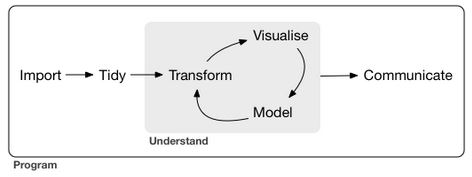
\includegraphics{workflow.jpg}
\caption{Illustration of workflow for data science}
\end{figure}

\hypertarget{import}{%
\subsubsection{Import}\label{import}}

Import is the first workflow stage that is required for the data science
project. The objective to achieve in import stage loading data into the
R data frame. The loaded will be used to perform data science in R. In
this case the Toyota dataset is available in Comma Separated Value .csv
file format. Using RStudio, ``readr'' package will be required to be
installed and loaded to library to add the dataset in the RStudio
environment. The skills required is to use R code ``read\_csv'' to read
the Toyota dataset. Possible challenges are that users may find RStudio
may unable to find the package in its library, thereby additional steps
need to be taken install ``readr'' or ``tidyverse'' package which
enables ``readr'' to be used.

\hypertarget{tidy}{%
\subsubsection{Tidy}\label{tidy}}

The next stage is to tidy up the data's in the dataset. The objective of
this stage is to tidy up data so that each column of the data is a
variable and each row of the data is an observation. The package that
will be useful for tidy stage is the ``janitor'' package which must be
loaded in RStudio. The skills required is to examine the Toyota dataset
for inconsistency and also skills to use functions in ``janitor''
package as required. Challenges that are faced is the time spent in
examining every single observation row for any inclusion of variables
especially for large datasets.

\hypertarget{transform}{%
\subsubsection{Transform}\label{transform}}

The objective of the transform stage is to narrow down the Toyota
dataset by creating a subset of the variables from the main dataset.
This subset of variables will be wrangled further to obtain desired
observation, statistic or outputs. The packages that will be used in
this stage is the ``dplyr'' package loaded in RStudio. The skills
required in this stage to successfully manipulate the variable using
``dplyr'' functions such as ``select()'' to generate narrowed down
variables dataset, ``filter()'' to extract data based constrain
parameters, ``rename()'' to create a new mutated variable and others
according model output requirement. The challenges faced is that wrong
manipulation could result in incorrect observation output and the
relationship between the outcome variable and predictors will not be
accurate. Another challenge is irrelevant variables are manipulated
resulting in desired output unable to be achieved.

\hypertarget{visualisation}{%
\subsubsection{Visualisation}\label{visualisation}}

Visualisation stage objective is to visualise the data for
interpretation. This will assist in identifying outliers, unexpected
data variability, and questioning unusual data. The required package for
this stage is the ``ggplot2'' package loaded in RStudio. The skill
required for this stage is the ability to spot outliers or interpret the
visualisation to identify the unusual data instances. The challenge is
the ability to identify data instances that are outliers.

\hypertarget{model}{%
\subsubsection{Model}\label{model}}

In model stage, the objective is to model applying multiple linear
regression on the selected outcome and predictor variable of the Toyota
dataset, tidying the result and assessing the model. The required
packages for this stages is the ``broom'' and ``kableExtra'' packages
which enables to use functions like ``augment()'', ``tidy()'',
``glance()'' and ``kable()'. The required skill is the ability to
understand why certain data point is much different with the rest. The
challenge is to determine what is the appropriate range for identifying
the outliers, as too many data instances could be disregarded if the
range parameter not determined appropriately.

\hypertarget{communication}{%
\subsubsection{Communication}\label{communication}}

Communication stage where the output results are interpreted and
communicated to others. The skill required is too interpret the
relationship between predictor variable and outcome variable based on
the results output. Challenge is correctly interpreting the estimate and
p value.

(585 words)

\hypertarget{analysis}{%
\section{Analysis}\label{analysis}}

\hypertarget{import-1}{%
\subsection{Import}\label{import-1}}

\hypertarget{load-libraries-to-do-analysis}{%
\subsubsection{Load libraries to do
analysis}\label{load-libraries-to-do-analysis}}

\begin{Shaded}
\begin{Highlighting}[]
\FunctionTok{library}\NormalTok{(tidyverse) }
\end{Highlighting}
\end{Shaded}

\begin{verbatim}
## -- Attaching packages --------------------------------------- tidyverse 1.3.1 --
\end{verbatim}

\begin{verbatim}
## v ggplot2 3.3.5     v purrr   0.3.4
## v tibble  3.1.2     v dplyr   1.0.7
## v tidyr   1.1.3     v stringr 1.4.0
## v readr   1.4.0     v forcats 0.5.1
\end{verbatim}

\begin{verbatim}
## -- Conflicts ------------------------------------------ tidyverse_conflicts() --
## x dplyr::filter() masks stats::filter()
## x dplyr::lag()    masks stats::lag()
\end{verbatim}

\begin{Shaded}
\begin{Highlighting}[]
\FunctionTok{library}\NormalTok{(janitor)}
\end{Highlighting}
\end{Shaded}

\begin{verbatim}
## 
## Attaching package: 'janitor'
\end{verbatim}

\begin{verbatim}
## The following objects are masked from 'package:stats':
## 
##     chisq.test, fisher.test
\end{verbatim}

\begin{Shaded}
\begin{Highlighting}[]
\FunctionTok{library}\NormalTok{(broom)}
\FunctionTok{library}\NormalTok{(readxl)}
\FunctionTok{library}\NormalTok{(kableExtra)}
\end{Highlighting}
\end{Shaded}

\begin{verbatim}
## 
## Attaching package: 'kableExtra'
\end{verbatim}

\begin{verbatim}
## The following object is masked from 'package:dplyr':
## 
##     group_rows
\end{verbatim}

\hypertarget{read-data-in-the-folder-of-project-directory}{%
\subsubsection{Read data in the folder of project
directory}\label{read-data-in-the-folder-of-project-directory}}

\begin{Shaded}
\begin{Highlighting}[]
\NormalTok{toyota }\OtherTok{\textless{}{-}} \FunctionTok{read\_csv}\NormalTok{(}\StringTok{\textquotesingle{}Toyota\_corolla.csv\textquotesingle{}}\NormalTok{)}
\end{Highlighting}
\end{Shaded}

\begin{verbatim}
## 
## -- Column specification --------------------------------------------------------
## cols(
##   .default = col_double(),
##   Model = col_character(),
##   Fuel_Type = col_character(),
##   Color = col_character()
## )
## i Use `spec()` for the full column specifications.
\end{verbatim}

\hypertarget{tidy-1}{%
\subsection{Tidy}\label{tidy-1}}

\hypertarget{clean-data}{%
\subsubsection{Clean data}\label{clean-data}}

\begin{Shaded}
\begin{Highlighting}[]
\NormalTok{toyota }\OtherTok{\textless{}{-}}\NormalTok{ toyota }\SpecialCharTok{\%\textgreater{}\%} 
  \FunctionTok{clean\_names}\NormalTok{()}
\end{Highlighting}
\end{Shaded}

\hypertarget{view-data}{%
\subsubsection{View data}\label{view-data}}

\begin{Shaded}
\begin{Highlighting}[]
\FunctionTok{summary}\NormalTok{(toyota)}
\end{Highlighting}
\end{Shaded}

\begin{verbatim}
##        id            model               price         age_08_04    
##  Min.   :   1.0   Length:1436        Min.   : 4350   Min.   : 1.00  
##  1st Qu.: 361.8   Class :character   1st Qu.: 8450   1st Qu.:44.00  
##  Median : 721.5   Mode  :character   Median : 9900   Median :61.00  
##  Mean   : 721.6                      Mean   :10731   Mean   :55.95  
##  3rd Qu.:1081.2                      3rd Qu.:11950   3rd Qu.:70.00  
##  Max.   :1442.0                      Max.   :32500   Max.   :80.00  
##    mfg_month         mfg_year          km          fuel_type        
##  Min.   : 1.000   Min.   :1998   Min.   :     1   Length:1436       
##  1st Qu.: 3.000   1st Qu.:1998   1st Qu.: 43000   Class :character  
##  Median : 5.000   Median :1999   Median : 63390   Mode  :character  
##  Mean   : 5.549   Mean   :2000   Mean   : 68533                     
##  3rd Qu.: 8.000   3rd Qu.:2001   3rd Qu.: 87021                     
##  Max.   :12.000   Max.   :2004   Max.   :243000                     
##        hp          met_color         color             automatic      
##  Min.   : 69.0   Min.   :0.0000   Length:1436        Min.   :0.00000  
##  1st Qu.: 90.0   1st Qu.:0.0000   Class :character   1st Qu.:0.00000  
##  Median :110.0   Median :1.0000   Mode  :character   Median :0.00000  
##  Mean   :101.5   Mean   :0.6748                      Mean   :0.05571  
##  3rd Qu.:110.0   3rd Qu.:1.0000                      3rd Qu.:0.00000  
##  Max.   :192.0   Max.   :1.0000                      Max.   :1.00000  
##        cc            doors         cylinders     gears       quarterly_tax   
##  Min.   : 1300   Min.   :2.000   Min.   :4   Min.   :3.000   Min.   : 19.00  
##  1st Qu.: 1400   1st Qu.:3.000   1st Qu.:4   1st Qu.:5.000   1st Qu.: 69.00  
##  Median : 1600   Median :4.000   Median :4   Median :5.000   Median : 85.00  
##  Mean   : 1577   Mean   :4.033   Mean   :4   Mean   :5.026   Mean   : 87.12  
##  3rd Qu.: 1600   3rd Qu.:5.000   3rd Qu.:4   3rd Qu.:5.000   3rd Qu.: 85.00  
##  Max.   :16000   Max.   :5.000   Max.   :4   Max.   :6.000   Max.   :283.00  
##      weight     mfr_guarantee    bovag_guarantee  guarantee_period
##  Min.   :1000   Min.   :0.0000   Min.   :0.0000   Min.   : 3.000  
##  1st Qu.:1040   1st Qu.:0.0000   1st Qu.:1.0000   1st Qu.: 3.000  
##  Median :1070   Median :0.0000   Median :1.0000   Median : 3.000  
##  Mean   :1072   Mean   :0.4095   Mean   :0.8955   Mean   : 3.815  
##  3rd Qu.:1085   3rd Qu.:1.0000   3rd Qu.:1.0000   3rd Qu.: 3.000  
##  Max.   :1615   Max.   :1.0000   Max.   :1.0000   Max.   :36.000  
##       abs            airbag_1         airbag_2          airco       
##  Min.   :0.0000   Min.   :0.0000   Min.   :0.0000   Min.   :0.0000  
##  1st Qu.:1.0000   1st Qu.:1.0000   1st Qu.:0.0000   1st Qu.:0.0000  
##  Median :1.0000   Median :1.0000   Median :1.0000   Median :1.0000  
##  Mean   :0.8134   Mean   :0.9708   Mean   :0.7228   Mean   :0.5084  
##  3rd Qu.:1.0000   3rd Qu.:1.0000   3rd Qu.:1.0000   3rd Qu.:1.0000  
##  Max.   :1.0000   Max.   :1.0000   Max.   :1.0000   Max.   :1.0000  
##  automatic_airco   boardcomputer      cd_player       central_lock   
##  Min.   :0.00000   Min.   :0.0000   Min.   :0.0000   Min.   :0.0000  
##  1st Qu.:0.00000   1st Qu.:0.0000   1st Qu.:0.0000   1st Qu.:0.0000  
##  Median :0.00000   Median :0.0000   Median :0.0000   Median :1.0000  
##  Mean   :0.05641   Mean   :0.2946   Mean   :0.2187   Mean   :0.5801  
##  3rd Qu.:0.00000   3rd Qu.:1.0000   3rd Qu.:0.0000   3rd Qu.:1.0000  
##  Max.   :1.00000   Max.   :1.0000   Max.   :1.0000   Max.   :1.0000  
##  powered_windows power_steering       radio          mistlamps    
##  Min.   :0.000   Min.   :0.0000   Min.   :0.0000   Min.   :0.000  
##  1st Qu.:0.000   1st Qu.:1.0000   1st Qu.:0.0000   1st Qu.:0.000  
##  Median :1.000   Median :1.0000   Median :0.0000   Median :0.000  
##  Mean   :0.562   Mean   :0.9777   Mean   :0.1462   Mean   :0.257  
##  3rd Qu.:1.000   3rd Qu.:1.0000   3rd Qu.:0.0000   3rd Qu.:1.000  
##  Max.   :1.000   Max.   :1.0000   Max.   :1.0000   Max.   :1.000  
##   sport_model     backseat_divider  metallic_rim    radio_cassette  
##  Min.   :0.0000   Min.   :0.0000   Min.   :0.0000   Min.   :0.0000  
##  1st Qu.:0.0000   1st Qu.:1.0000   1st Qu.:0.0000   1st Qu.:0.0000  
##  Median :0.0000   Median :1.0000   Median :0.0000   Median :0.0000  
##  Mean   :0.3001   Mean   :0.7702   Mean   :0.2047   Mean   :0.1455  
##  3rd Qu.:1.0000   3rd Qu.:1.0000   3rd Qu.:0.0000   3rd Qu.:0.0000  
##  Max.   :1.0000   Max.   :1.0000   Max.   :1.0000   Max.   :1.0000  
##  parking_assistant     tow_bar      
##  Min.   :0.000000   Min.   :0.0000  
##  1st Qu.:0.000000   1st Qu.:0.0000  
##  Median :0.000000   Median :0.0000  
##  Mean   :0.002786   Mean   :0.2779  
##  3rd Qu.:0.000000   3rd Qu.:1.0000  
##  Max.   :1.000000   Max.   :1.0000
\end{verbatim}

\hypertarget{transform-1}{%
\subsection{Transform}\label{transform-1}}

\hypertarget{select-variable}{%
\subsubsection{Select variable}\label{select-variable}}

\hypertarget{model-a-1}{%
\paragraph{Model A}\label{model-a-1}}

\begin{Shaded}
\begin{Highlighting}[]
\NormalTok{toyotaA }\OtherTok{\textless{}{-}}\NormalTok{ toyota }\SpecialCharTok{\%\textgreater{}\%} 
  \FunctionTok{select}\NormalTok{(id, price, age\_08\_04, km, fuel\_type, met\_color, weight)}
\FunctionTok{glimpse}\NormalTok{(toyotaA)}
\end{Highlighting}
\end{Shaded}

\begin{verbatim}
## Rows: 1,436
## Columns: 7
## $ id        <dbl> 1, 2, 3, 4, 5, 6, 7, 8, 9, 10, 11, 12, 13, 14, 15, 16, 17, 1~
## $ price     <dbl> 13500, 13750, 13950, 14950, 13750, 12950, 16900, 18600, 2150~
## $ age_08_04 <dbl> 23, 23, 24, 26, 30, 32, 27, 30, 27, 23, 25, 22, 25, 31, 32, ~
## $ km        <dbl> 46986, 72937, 41711, 48000, 38500, 61000, 94612, 75889, 1970~
## $ fuel_type <chr> "Diesel", "Diesel", "Diesel", "Diesel", "Diesel", "Diesel", ~
## $ met_color <dbl> 1, 1, 1, 0, 0, 0, 1, 1, 0, 0, 0, 0, 0, 1, 1, 0, 1, 1, 0, 1, ~
## $ weight    <dbl> 1165, 1165, 1165, 1165, 1170, 1170, 1245, 1245, 1185, 1105, ~
\end{verbatim}

\hypertarget{model-b-1}{%
\paragraph{Model B}\label{model-b-1}}

\begin{Shaded}
\begin{Highlighting}[]
\NormalTok{toyotaB }\OtherTok{\textless{}{-}}\NormalTok{ toyota }\SpecialCharTok{\%\textgreater{}\%} 
  \FunctionTok{select}\NormalTok{(id, price, age\_08\_04, km, fuel\_type, cc, automatic)}
\FunctionTok{glimpse}\NormalTok{(toyotaB)}
\end{Highlighting}
\end{Shaded}

\begin{verbatim}
## Rows: 1,436
## Columns: 7
## $ id        <dbl> 1, 2, 3, 4, 5, 6, 7, 8, 9, 10, 11, 12, 13, 14, 15, 16, 17, 1~
## $ price     <dbl> 13500, 13750, 13950, 14950, 13750, 12950, 16900, 18600, 2150~
## $ age_08_04 <dbl> 23, 23, 24, 26, 30, 32, 27, 30, 27, 23, 25, 22, 25, 31, 32, ~
## $ km        <dbl> 46986, 72937, 41711, 48000, 38500, 61000, 94612, 75889, 1970~
## $ fuel_type <chr> "Diesel", "Diesel", "Diesel", "Diesel", "Diesel", "Diesel", ~
## $ cc        <dbl> 2000, 2000, 2000, 2000, 2000, 2000, 2000, 2000, 1800, 1900, ~
## $ automatic <dbl> 0, 0, 0, 0, 0, 0, 0, 0, 0, 0, 0, 0, 0, 0, 0, 0, 0, 0, 0, 0, ~
\end{verbatim}

\hypertarget{model-c-1}{%
\paragraph{Model C}\label{model-c-1}}

\begin{Shaded}
\begin{Highlighting}[]
\NormalTok{toyotaC }\OtherTok{\textless{}{-}}\NormalTok{ toyota }\SpecialCharTok{\%\textgreater{}\%} 
  \FunctionTok{select}\NormalTok{(id, price, age\_08\_04, km, hp, abs, airco)}
\FunctionTok{glimpse}\NormalTok{(toyotaC)}
\end{Highlighting}
\end{Shaded}

\begin{verbatim}
## Rows: 1,436
## Columns: 7
## $ id        <dbl> 1, 2, 3, 4, 5, 6, 7, 8, 9, 10, 11, 12, 13, 14, 15, 16, 17, 1~
## $ price     <dbl> 13500, 13750, 13950, 14950, 13750, 12950, 16900, 18600, 2150~
## $ age_08_04 <dbl> 23, 23, 24, 26, 30, 32, 27, 30, 27, 23, 25, 22, 25, 31, 32, ~
## $ km        <dbl> 46986, 72937, 41711, 48000, 38500, 61000, 94612, 75889, 1970~
## $ hp        <dbl> 90, 90, 90, 90, 90, 90, 90, 90, 192, 69, 192, 192, 192, 192,~
## $ abs       <dbl> 1, 1, 1, 1, 1, 1, 1, 1, 1, 1, 1, 1, 1, 1, 1, 1, 1, 1, 1, 1, ~
## $ airco     <dbl> 0, 1, 0, 0, 1, 1, 1, 1, 1, 1, 1, 1, 1, 1, 1, 1, 1, 1, 1, 1, ~
\end{verbatim}

\hypertarget{mutate-variables}{%
\subsubsection{Mutate variables}\label{mutate-variables}}

\hypertarget{model-a-2}{%
\paragraph{Model A}\label{model-a-2}}

\begin{Shaded}
\begin{Highlighting}[]
\NormalTok{toyotaA }\OtherTok{\textless{}{-}}\NormalTok{ toyotaA }\SpecialCharTok{\%\textgreater{}\%} 
  \FunctionTok{mutate}\NormalTok{(}\AttributeTok{met\_color =} \FunctionTok{factor}\NormalTok{(met\_color,}
                              \AttributeTok{label =} \FunctionTok{c}\NormalTok{(}\StringTok{\textquotesingle{}No\textquotesingle{}}\NormalTok{, }\StringTok{\textquotesingle{}Yes\textquotesingle{}}\NormalTok{)))}
\end{Highlighting}
\end{Shaded}

\hypertarget{model-b-2}{%
\paragraph{Model B}\label{model-b-2}}

\begin{Shaded}
\begin{Highlighting}[]
\NormalTok{toyotaB }\OtherTok{\textless{}{-}}\NormalTok{ toyotaB }\SpecialCharTok{\%\textgreater{}\%} 
  \FunctionTok{mutate}\NormalTok{(}\AttributeTok{automatic =} \FunctionTok{factor}\NormalTok{(automatic,}
                              \AttributeTok{label =} \FunctionTok{c}\NormalTok{(}\StringTok{\textquotesingle{}No\textquotesingle{}}\NormalTok{, }\StringTok{\textquotesingle{}Yes\textquotesingle{}}\NormalTok{)))}
\end{Highlighting}
\end{Shaded}

\hypertarget{model-c-2}{%
\paragraph{Model C}\label{model-c-2}}

\begin{Shaded}
\begin{Highlighting}[]
\NormalTok{toyotaC }\OtherTok{\textless{}{-}}\NormalTok{ toyotaC }\SpecialCharTok{\%\textgreater{}\%}
  \FunctionTok{mutate}\NormalTok{(}\AttributeTok{abs =} \FunctionTok{factor}\NormalTok{(abs,}
                      \AttributeTok{label =} \FunctionTok{c}\NormalTok{(}\StringTok{\textquotesingle{}No\textquotesingle{}}\NormalTok{, }\StringTok{\textquotesingle{}Yes\textquotesingle{}}\NormalTok{)))}
\end{Highlighting}
\end{Shaded}

\begin{Shaded}
\begin{Highlighting}[]
\NormalTok{toyotaC }\OtherTok{\textless{}{-}}\NormalTok{ toyotaC }\SpecialCharTok{\%\textgreater{}\%}
  \FunctionTok{mutate}\NormalTok{(}\AttributeTok{airco =} \FunctionTok{factor}\NormalTok{(airco,}
                      \AttributeTok{label =} \FunctionTok{c}\NormalTok{(}\StringTok{\textquotesingle{}No\textquotesingle{}}\NormalTok{, }\StringTok{\textquotesingle{}Yes\textquotesingle{}}\NormalTok{)))}
\end{Highlighting}
\end{Shaded}

\hypertarget{section-4}{%
\subsection{Section 4}\label{section-4}}

\hypertarget{categorize-a-numerical-variable-and-regroup-a-categorical-variable}{%
\subsubsection{Categorize a numerical variable and regroup a categorical
variable}\label{categorize-a-numerical-variable-and-regroup-a-categorical-variable}}

\hypertarget{model-a-3}{%
\paragraph{Model A}\label{model-a-3}}

\begin{Shaded}
\begin{Highlighting}[]
\NormalTok{toyotaA }\OtherTok{\textless{}{-}}\NormalTok{ toyotaA }\SpecialCharTok{\%\textgreater{}\%}
  \FunctionTok{mutate}\NormalTok{(}\AttributeTok{catA =} \FunctionTok{cut}\NormalTok{(weight,}
                    \AttributeTok{breaks =} \FunctionTok{c}\NormalTok{(}\DecValTok{0}\NormalTok{, }\DecValTok{1134}\NormalTok{, }\DecValTok{1360}\NormalTok{, }\DecValTok{1587}\NormalTok{, }\DecValTok{1814}\NormalTok{),}
                    \AttributeTok{labels =} \FunctionTok{c}\NormalTok{(}\StringTok{\textquotesingle{}Passenger cars light\textquotesingle{}}\NormalTok{, }\StringTok{\textquotesingle{}Passenger cars compact\textquotesingle{}}\NormalTok{, }\StringTok{\textquotesingle{}Passenger cars medium\textquotesingle{}}\NormalTok{, }\StringTok{\textquotesingle{}Passenger cars heavy\textquotesingle{}}\NormalTok{)))}
\end{Highlighting}
\end{Shaded}

The cut points for the weight variable in model A is chosen due to the
cut points being the vehicle size classes of the National Highway
Traffic Safety Administrations (NHTSA). This weight classes are used as
the standard for New Car Assessment Program (NCAP) testing in United
States (U.S.). The cuts point for passenger cars according to the
standard; light, above 907kg to below 1134kg; compact, up to 1360kg,
medium, up to 1587kg; and heavy, up to 1814kg. The changes to the model
parameters are the weight variable was initially a numerical variable.
Now the mutated categorical variable catA will result in the multiple
linear regression model to have the cut points category to be referenced
to the dummy category of ``Passenger cars light''.

(124 words)

\hypertarget{model-b-3}{%
\paragraph{Model B}\label{model-b-3}}

\begin{Shaded}
\begin{Highlighting}[]
\NormalTok{toyotaB }\OtherTok{\textless{}{-}}\NormalTok{ toyotaB }\SpecialCharTok{\%\textgreater{}\%}
  \FunctionTok{mutate}\NormalTok{(}\AttributeTok{catB =} \FunctionTok{recode}\NormalTok{(fuel\_type,}
                       \StringTok{\textquotesingle{}Diesel\textquotesingle{}} \OtherTok{=} \StringTok{\textquotesingle{}liquid fuel\textquotesingle{}}\NormalTok{,}
                       \StringTok{\textquotesingle{}Petrol\textquotesingle{}} \OtherTok{=} \StringTok{\textquotesingle{}liquid fuel\textquotesingle{}}\NormalTok{,}
                       \StringTok{\textquotesingle{}CNG\textquotesingle{}} \OtherTok{=} \StringTok{\textquotesingle{}fuel gas\textquotesingle{}}\NormalTok{))}
\end{Highlighting}
\end{Shaded}

The new categories are chosen so that the fuel types can be segregated
by liquid fuel and fuel gas. These two particular categories were chosen
to investigate the impact of having gas cylinders on vehicle price. The
fuel gas requires gas tanks to be installed in the boot of sedans such
as Toyota corolla in our case, which will limit the boot space. This
could potentially have a negative impact on the price of the vehicle.
The changes to the model parameters is that now Model B's multiple
linear regression model predictor variable catB which replaces
fuel\_type, will only have `liquid fuel' as a reference category to
dummy category `fuel gas'.

(111 words)

\hypertarget{view-data-1}{%
\subsubsection{View data}\label{view-data-1}}

\hypertarget{model-a-4}{%
\paragraph{Model A}\label{model-a-4}}

\begin{Shaded}
\begin{Highlighting}[]
\FunctionTok{summary}\NormalTok{(toyotaA)}
\end{Highlighting}
\end{Shaded}

\begin{verbatim}
##        id             price         age_08_04           km        
##  Min.   :   1.0   Min.   : 4350   Min.   : 1.00   Min.   :     1  
##  1st Qu.: 361.8   1st Qu.: 8450   1st Qu.:44.00   1st Qu.: 43000  
##  Median : 721.5   Median : 9900   Median :61.00   Median : 63390  
##  Mean   : 721.6   Mean   :10731   Mean   :55.95   Mean   : 68533  
##  3rd Qu.:1081.2   3rd Qu.:11950   3rd Qu.:70.00   3rd Qu.: 87021  
##  Max.   :1442.0   Max.   :32500   Max.   :80.00   Max.   :243000  
##   fuel_type         met_color     weight                         catA     
##  Length:1436        No :467   Min.   :1000   Passenger cars light  :1314  
##  Class :character   Yes:969   1st Qu.:1040   Passenger cars compact: 117  
##  Mode  :character             Median :1070   Passenger cars medium :   4  
##                               Mean   :1072   Passenger cars heavy  :   1  
##                               3rd Qu.:1085                                
##                               Max.   :1615
\end{verbatim}

\hypertarget{model-b-4}{%
\paragraph{Model B}\label{model-b-4}}

\begin{Shaded}
\begin{Highlighting}[]
\FunctionTok{summary}\NormalTok{(toyotaB)}
\end{Highlighting}
\end{Shaded}

\begin{verbatim}
##        id             price         age_08_04           km        
##  Min.   :   1.0   Min.   : 4350   Min.   : 1.00   Min.   :     1  
##  1st Qu.: 361.8   1st Qu.: 8450   1st Qu.:44.00   1st Qu.: 43000  
##  Median : 721.5   Median : 9900   Median :61.00   Median : 63390  
##  Mean   : 721.6   Mean   :10731   Mean   :55.95   Mean   : 68533  
##  3rd Qu.:1081.2   3rd Qu.:11950   3rd Qu.:70.00   3rd Qu.: 87021  
##  Max.   :1442.0   Max.   :32500   Max.   :80.00   Max.   :243000  
##   fuel_type               cc        automatic      catB          
##  Length:1436        Min.   : 1300   No :1356   Length:1436       
##  Class :character   1st Qu.: 1400   Yes:  80   Class :character  
##  Mode  :character   Median : 1600              Mode  :character  
##                     Mean   : 1577                                
##                     3rd Qu.: 1600                                
##                     Max.   :16000
\end{verbatim}

\hypertarget{model-c-3}{%
\paragraph{Model C}\label{model-c-3}}

\begin{Shaded}
\begin{Highlighting}[]
\FunctionTok{summary}\NormalTok{(toyotaC)}
\end{Highlighting}
\end{Shaded}

\begin{verbatim}
##        id             price         age_08_04           km        
##  Min.   :   1.0   Min.   : 4350   Min.   : 1.00   Min.   :     1  
##  1st Qu.: 361.8   1st Qu.: 8450   1st Qu.:44.00   1st Qu.: 43000  
##  Median : 721.5   Median : 9900   Median :61.00   Median : 63390  
##  Mean   : 721.6   Mean   :10731   Mean   :55.95   Mean   : 68533  
##  3rd Qu.:1081.2   3rd Qu.:11950   3rd Qu.:70.00   3rd Qu.: 87021  
##  Max.   :1442.0   Max.   :32500   Max.   :80.00   Max.   :243000  
##        hp         abs       airco    
##  Min.   : 69.0   No : 268   No :706  
##  1st Qu.: 90.0   Yes:1168   Yes:730  
##  Median :110.0                       
##  Mean   :101.5                       
##  3rd Qu.:110.0                       
##  Max.   :192.0
\end{verbatim}

\hypertarget{exploratory-data-analysis-eda}{%
\subparagraph{Exploratory data analysis
(EDA)}\label{exploratory-data-analysis-eda}}

\hypertarget{summarize-data}{%
\subsubsection{Summarize data}\label{summarize-data}}

\hypertarget{model-a-5}{%
\paragraph{Model A}\label{model-a-5}}

\begin{Shaded}
\begin{Highlighting}[]
\FunctionTok{options}\NormalTok{(}\AttributeTok{scipen =} \DecValTok{999}\NormalTok{) }
\NormalTok{toyotaA }\SpecialCharTok{\%\textgreater{}\%} \FunctionTok{summarize}\NormalTok{(}\AttributeTok{mean\_age =} \FunctionTok{mean}\NormalTok{(age\_08\_04, }\AttributeTok{na.rm =}\NormalTok{ T),}
                      \AttributeTok{mean\_KM =} \FunctionTok{mean}\NormalTok{(km, }\AttributeTok{na.rm =}\NormalTok{ T),}
                      \AttributeTok{mean\_Weight =} \FunctionTok{mean}\NormalTok{(weight, }\AttributeTok{na.rm =}\NormalTok{ T),}
                      \AttributeTok{sd\_age =} \FunctionTok{sd}\NormalTok{(age\_08\_04, }\AttributeTok{na.rm =}\NormalTok{ T),}
                      \AttributeTok{sd\_KM =} \FunctionTok{sd}\NormalTok{(km, }\AttributeTok{na.rm =}\NormalTok{ T),}
                      \AttributeTok{sd\_Weight =} \FunctionTok{sd}\NormalTok{(weight, }\AttributeTok{na.rm =}\NormalTok{ T)) }\SpecialCharTok{\%\textgreater{}\%} 
  \FunctionTok{gather}\NormalTok{()}
\end{Highlighting}
\end{Shaded}

\begin{verbatim}
## # A tibble: 6 x 2
##   key           value
##   <chr>         <dbl>
## 1 mean_age       55.9
## 2 mean_KM     68533. 
## 3 mean_Weight  1072. 
## 4 sd_age         18.6
## 5 sd_KM       37506. 
## 6 sd_Weight      52.6
\end{verbatim}

\hypertarget{model-b-5}{%
\paragraph{Model B}\label{model-b-5}}

\begin{Shaded}
\begin{Highlighting}[]
\FunctionTok{options}\NormalTok{(}\AttributeTok{scipen =} \DecValTok{999}\NormalTok{) }
\NormalTok{toyotaB }\SpecialCharTok{\%\textgreater{}\%} \FunctionTok{summarize}\NormalTok{(}\AttributeTok{mean\_age =} \FunctionTok{mean}\NormalTok{(age\_08\_04, }\AttributeTok{na.rm =}\NormalTok{ T),}
                      \AttributeTok{mean\_KM =} \FunctionTok{mean}\NormalTok{(km, }\AttributeTok{na.rm =}\NormalTok{ T),}
                      \AttributeTok{mean\_cc =} \FunctionTok{mean}\NormalTok{(cc, }\AttributeTok{na.rm =}\NormalTok{ T),}
                      \AttributeTok{sd\_age =} \FunctionTok{sd}\NormalTok{(age\_08\_04, }\AttributeTok{na.rm =}\NormalTok{ T),}
                      \AttributeTok{sd\_KM =} \FunctionTok{sd}\NormalTok{(km, }\AttributeTok{na.rm =}\NormalTok{ T),}
                      \AttributeTok{sd\_cc =} \FunctionTok{sd}\NormalTok{(cc, }\AttributeTok{na.rm =}\NormalTok{ T)) }\SpecialCharTok{\%\textgreater{}\%} 
  \FunctionTok{gather}\NormalTok{()}
\end{Highlighting}
\end{Shaded}

\begin{verbatim}
## # A tibble: 6 x 2
##   key        value
##   <chr>      <dbl>
## 1 mean_age    55.9
## 2 mean_KM  68533. 
## 3 mean_cc   1577. 
## 4 sd_age      18.6
## 5 sd_KM    37506. 
## 6 sd_cc      424.
\end{verbatim}

\hypertarget{model-c-4}{%
\paragraph{Model C}\label{model-c-4}}

\begin{Shaded}
\begin{Highlighting}[]
\FunctionTok{options}\NormalTok{(}\AttributeTok{scipen =} \DecValTok{999}\NormalTok{) }
\NormalTok{toyotaC }\SpecialCharTok{\%\textgreater{}\%} \FunctionTok{summarize}\NormalTok{(}\AttributeTok{mean\_age =} \FunctionTok{mean}\NormalTok{(age\_08\_04, }\AttributeTok{na.rm =}\NormalTok{ T),}
                      \AttributeTok{mean\_KM =} \FunctionTok{mean}\NormalTok{(km, }\AttributeTok{na.rm =}\NormalTok{ T),}
                      \AttributeTok{mean\_hp =} \FunctionTok{mean}\NormalTok{(hp, }\AttributeTok{na.rm =}\NormalTok{ T),}
                      \AttributeTok{sd\_age =} \FunctionTok{sd}\NormalTok{(age\_08\_04, }\AttributeTok{na.rm =}\NormalTok{ T),}
                      \AttributeTok{sd\_KM =} \FunctionTok{sd}\NormalTok{(km, }\AttributeTok{na.rm =}\NormalTok{ T),}
                      \AttributeTok{sd\_hp =} \FunctionTok{sd}\NormalTok{(hp, }\AttributeTok{na.rm =}\NormalTok{ T)) }\SpecialCharTok{\%\textgreater{}\%} 
  \FunctionTok{gather}\NormalTok{()}
\end{Highlighting}
\end{Shaded}

\begin{verbatim}
## # A tibble: 6 x 2
##   key        value
##   <chr>      <dbl>
## 1 mean_age    55.9
## 2 mean_KM  68533. 
## 3 mean_hp    102. 
## 4 sd_age      18.6
## 5 sd_KM    37506. 
## 6 sd_hp       15.0
\end{verbatim}

\hypertarget{visualise}{%
\subsection{Visualise}\label{visualise}}

\hypertarget{model-a-6}{%
\paragraph{Model A}\label{model-a-6}}

Age of cars

\begin{Shaded}
\begin{Highlighting}[]
\FunctionTok{ggplot}\NormalTok{(toyotaA, }\FunctionTok{aes}\NormalTok{(age\_08\_04)) }\SpecialCharTok{+} \FunctionTok{geom\_histogram}\NormalTok{(}\AttributeTok{color=}\StringTok{"\#99CC00"}\NormalTok{, }\AttributeTok{fill=}\StringTok{"\#99CC00"}\NormalTok{)}
\end{Highlighting}
\end{Shaded}

\begin{verbatim}
## `stat_bin()` using `bins = 30`. Pick better value with `binwidth`.
\end{verbatim}

\includegraphics{Toyota-analysis_files/figure-latex/unnamed-chunk-20-1.pdf}

Mileage

\begin{Shaded}
\begin{Highlighting}[]
\FunctionTok{ggplot}\NormalTok{(toyotaA, }\FunctionTok{aes}\NormalTok{(km)) }\SpecialCharTok{+} \FunctionTok{geom\_histogram}\NormalTok{(}\AttributeTok{color=}\StringTok{"lightblue"}\NormalTok{, }\AttributeTok{fill=}\StringTok{"lightblue"}\NormalTok{) }
\end{Highlighting}
\end{Shaded}

\begin{verbatim}
## `stat_bin()` using `bins = 30`. Pick better value with `binwidth`.
\end{verbatim}

\includegraphics{Toyota-analysis_files/figure-latex/unnamed-chunk-21-1.pdf}

Metallic colour, Fuel type, catA (Count)

\begin{Shaded}
\begin{Highlighting}[]
\NormalTok{toyotaA }\SpecialCharTok{\%\textgreater{}\%} 
  \FunctionTok{count}\NormalTok{(met\_color, fuel\_type, catA)}
\end{Highlighting}
\end{Shaded}

\begin{verbatim}
## # A tibble: 14 x 4
##    met_color fuel_type catA                       n
##    <fct>     <chr>     <fct>                  <int>
##  1 No        CNG       Passenger cars light       4
##  2 No        Diesel    Passenger cars light      26
##  3 No        Diesel    Passenger cars compact    26
##  4 No        Diesel    Passenger cars medium      1
##  5 No        Petrol    Passenger cars light     399
##  6 No        Petrol    Passenger cars compact    10
##  7 No        Petrol    Passenger cars medium      1
##  8 Yes       CNG       Passenger cars light      13
##  9 Yes       Diesel    Passenger cars light      34
## 10 Yes       Diesel    Passenger cars compact    66
## 11 Yes       Diesel    Passenger cars medium      2
## 12 Yes       Petrol    Passenger cars light     838
## 13 Yes       Petrol    Passenger cars compact    15
## 14 Yes       Petrol    Passenger cars heavy       1
\end{verbatim}

Fuel type (count) plot

\begin{Shaded}
\begin{Highlighting}[]
\FunctionTok{ggplot}\NormalTok{(toyotaA, }\FunctionTok{aes}\NormalTok{(fuel\_type)) }\SpecialCharTok{+} \FunctionTok{geom\_bar}\NormalTok{(}\AttributeTok{color=}\StringTok{"lightpink"}\NormalTok{, }\AttributeTok{fill=}\StringTok{"lightpink"}\NormalTok{) }
\end{Highlighting}
\end{Shaded}

\includegraphics{Toyota-analysis_files/figure-latex/unnamed-chunk-23-1.pdf}

Metallic color (count)plot

\begin{Shaded}
\begin{Highlighting}[]
\FunctionTok{ggplot}\NormalTok{(toyotaA, }\FunctionTok{aes}\NormalTok{(met\_color)) }\SpecialCharTok{+} \FunctionTok{geom\_bar}\NormalTok{(}\AttributeTok{color=}\StringTok{"\#996666"}\NormalTok{, }\AttributeTok{fill=}\StringTok{"\#996666"}\NormalTok{)}
\end{Highlighting}
\end{Shaded}

\includegraphics{Toyota-analysis_files/figure-latex/unnamed-chunk-24-1.pdf}

Metallic color (count)plot

\begin{Shaded}
\begin{Highlighting}[]
\FunctionTok{ggplot}\NormalTok{(toyotaA, }\FunctionTok{aes}\NormalTok{(catA)) }\SpecialCharTok{+} \FunctionTok{geom\_bar}\NormalTok{(}\AttributeTok{color=}\StringTok{"orange"}\NormalTok{, }\AttributeTok{fill=}\StringTok{"orange"}\NormalTok{)}
\end{Highlighting}
\end{Shaded}

\includegraphics{Toyota-analysis_files/figure-latex/unnamed-chunk-25-1.pdf}

\hypertarget{model-b-6}{%
\paragraph{Model B}\label{model-b-6}}

Age of cars

\begin{Shaded}
\begin{Highlighting}[]
\FunctionTok{ggplot}\NormalTok{(toyotaB, }\FunctionTok{aes}\NormalTok{(age\_08\_04)) }\SpecialCharTok{+} \FunctionTok{geom\_histogram}\NormalTok{(}\AttributeTok{color=}\StringTok{"\#99CC00"}\NormalTok{, }\AttributeTok{fill=}\StringTok{"\#99CC00"}\NormalTok{)}
\end{Highlighting}
\end{Shaded}

\begin{verbatim}
## `stat_bin()` using `bins = 30`. Pick better value with `binwidth`.
\end{verbatim}

\includegraphics{Toyota-analysis_files/figure-latex/unnamed-chunk-26-1.pdf}

Mileage

\begin{Shaded}
\begin{Highlighting}[]
\FunctionTok{ggplot}\NormalTok{(toyotaB, }\FunctionTok{aes}\NormalTok{(km)) }\SpecialCharTok{+} \FunctionTok{geom\_histogram}\NormalTok{(}\AttributeTok{color=}\StringTok{"lightblue"}\NormalTok{, }\AttributeTok{fill=}\StringTok{"lightblue"}\NormalTok{) }
\end{Highlighting}
\end{Shaded}

\begin{verbatim}
## `stat_bin()` using `bins = 30`. Pick better value with `binwidth`.
\end{verbatim}

\includegraphics{Toyota-analysis_files/figure-latex/unnamed-chunk-27-1.pdf}

Engine size, cc

\begin{Shaded}
\begin{Highlighting}[]
\FunctionTok{ggplot}\NormalTok{(toyotaB, }\FunctionTok{aes}\NormalTok{(cc)) }\SpecialCharTok{+} \FunctionTok{geom\_histogram}\NormalTok{(}\AttributeTok{color=}\StringTok{"\#FFCC00"}\NormalTok{, }\AttributeTok{fill=}\StringTok{"\#FFCC00"}\NormalTok{)}
\end{Highlighting}
\end{Shaded}

\begin{verbatim}
## `stat_bin()` using `bins = 30`. Pick better value with `binwidth`.
\end{verbatim}

\includegraphics{Toyota-analysis_files/figure-latex/unnamed-chunk-28-1.pdf}

Automatic, CatB (Count)

\begin{Shaded}
\begin{Highlighting}[]
\NormalTok{toyotaB }\SpecialCharTok{\%\textgreater{}\%} 
  \FunctionTok{count}\NormalTok{(automatic, catB)}
\end{Highlighting}
\end{Shaded}

\begin{verbatim}
## # A tibble: 4 x 3
##   automatic catB            n
##   <fct>     <chr>       <int>
## 1 No        fuel gas       16
## 2 No        liquid fuel  1340
## 3 Yes       fuel gas        1
## 4 Yes       liquid fuel    79
\end{verbatim}

catB (count) plot

\begin{Shaded}
\begin{Highlighting}[]
\FunctionTok{ggplot}\NormalTok{(toyotaB, }\FunctionTok{aes}\NormalTok{(catB)) }\SpecialCharTok{+} \FunctionTok{geom\_bar}\NormalTok{(}\AttributeTok{color=}\StringTok{"lightpink"}\NormalTok{, }\AttributeTok{fill=}\StringTok{"lightpink"}\NormalTok{) }
\end{Highlighting}
\end{Shaded}

\includegraphics{Toyota-analysis_files/figure-latex/unnamed-chunk-30-1.pdf}

Automatic (count) plot

\begin{Shaded}
\begin{Highlighting}[]
\FunctionTok{ggplot}\NormalTok{(toyotaB, }\FunctionTok{aes}\NormalTok{(automatic)) }\SpecialCharTok{+} \FunctionTok{geom\_bar}\NormalTok{(}\AttributeTok{color=}\StringTok{"\#996666"}\NormalTok{, }\AttributeTok{fill=}\StringTok{"\#996666"}\NormalTok{)}
\end{Highlighting}
\end{Shaded}

\includegraphics{Toyota-analysis_files/figure-latex/unnamed-chunk-31-1.pdf}

\hypertarget{model-c-5}{%
\paragraph{Model C}\label{model-c-5}}

Age of cars

\begin{Shaded}
\begin{Highlighting}[]
\FunctionTok{ggplot}\NormalTok{(toyotaC, }\FunctionTok{aes}\NormalTok{(age\_08\_04)) }\SpecialCharTok{+} \FunctionTok{geom\_histogram}\NormalTok{(}\AttributeTok{color=}\StringTok{"\#99CC00"}\NormalTok{, }\AttributeTok{fill=}\StringTok{"\#99CC00"}\NormalTok{)}
\end{Highlighting}
\end{Shaded}

\begin{verbatim}
## `stat_bin()` using `bins = 30`. Pick better value with `binwidth`.
\end{verbatim}

\includegraphics{Toyota-analysis_files/figure-latex/unnamed-chunk-32-1.pdf}

Mileage

\begin{Shaded}
\begin{Highlighting}[]
\FunctionTok{ggplot}\NormalTok{(toyotaC, }\FunctionTok{aes}\NormalTok{(km)) }\SpecialCharTok{+} \FunctionTok{geom\_histogram}\NormalTok{(}\AttributeTok{color=}\StringTok{"lightblue"}\NormalTok{, }\AttributeTok{fill=}\StringTok{"lightblue"}\NormalTok{) }
\end{Highlighting}
\end{Shaded}

\begin{verbatim}
## `stat_bin()` using `bins = 30`. Pick better value with `binwidth`.
\end{verbatim}

\includegraphics{Toyota-analysis_files/figure-latex/unnamed-chunk-33-1.pdf}

Horsepower

\begin{Shaded}
\begin{Highlighting}[]
\FunctionTok{ggplot}\NormalTok{(toyotaC, }\FunctionTok{aes}\NormalTok{(hp)) }\SpecialCharTok{+} \FunctionTok{geom\_histogram}\NormalTok{(}\AttributeTok{color=}\StringTok{"\#FF6666"}\NormalTok{, }\AttributeTok{fill=}\StringTok{"\#FF6666"}\NormalTok{) }
\end{Highlighting}
\end{Shaded}

\begin{verbatim}
## `stat_bin()` using `bins = 30`. Pick better value with `binwidth`.
\end{verbatim}

\includegraphics{Toyota-analysis_files/figure-latex/unnamed-chunk-34-1.pdf}

Anti-lock braking system, air-conditioning (Count)

\begin{Shaded}
\begin{Highlighting}[]
\NormalTok{toyotaC }\SpecialCharTok{\%\textgreater{}\%} 
  \FunctionTok{count}\NormalTok{(abs, airco)}
\end{Highlighting}
\end{Shaded}

\begin{verbatim}
## # A tibble: 4 x 3
##   abs   airco     n
##   <fct> <fct> <int>
## 1 No    No      195
## 2 No    Yes      73
## 3 Yes   No      511
## 4 Yes   Yes     657
\end{verbatim}

Anti-lock braking system (count) plot

\begin{Shaded}
\begin{Highlighting}[]
\FunctionTok{ggplot}\NormalTok{(toyotaC, }\FunctionTok{aes}\NormalTok{(abs)) }\SpecialCharTok{+} \FunctionTok{geom\_bar}\NormalTok{(}\AttributeTok{color=}\StringTok{"\#99CCCC"}\NormalTok{, }\AttributeTok{fill=}\StringTok{"\#99CCCC"}\NormalTok{) }
\end{Highlighting}
\end{Shaded}

\includegraphics{Toyota-analysis_files/figure-latex/unnamed-chunk-36-1.pdf}

Air-conditioning (count)plot

\begin{Shaded}
\begin{Highlighting}[]
\FunctionTok{ggplot}\NormalTok{(toyotaC, }\FunctionTok{aes}\NormalTok{(airco)) }\SpecialCharTok{+} \FunctionTok{geom\_bar}\NormalTok{(}\AttributeTok{color=}\StringTok{"\#6699FF"}\NormalTok{, }\AttributeTok{fill=}\StringTok{"\#6699FF"}\NormalTok{)}
\end{Highlighting}
\end{Shaded}

\includegraphics{Toyota-analysis_files/figure-latex/unnamed-chunk-37-1.pdf}

\hypertarget{model-1}{%
\subsection{Model}\label{model-1}}

\hypertarget{multiple-linear-regression}{%
\subsubsection{Multiple Linear
Regression}\label{multiple-linear-regression}}

\hypertarget{model-a-7}{%
\paragraph{Model A}\label{model-a-7}}

\begin{Shaded}
\begin{Highlighting}[]
\NormalTok{modA\_mlr }\OtherTok{\textless{}{-}} \FunctionTok{lm}\NormalTok{(price }\SpecialCharTok{\textasciitilde{}}\NormalTok{ age\_08\_04 }\SpecialCharTok{+}\NormalTok{ km }\SpecialCharTok{+}\NormalTok{ fuel\_type }\SpecialCharTok{+} 
\NormalTok{                met\_color }\SpecialCharTok{+}\NormalTok{ catA, }\AttributeTok{data =}\NormalTok{ toyotaA)}
\end{Highlighting}
\end{Shaded}

\hypertarget{model-b-7}{%
\paragraph{Model B}\label{model-b-7}}

\begin{Shaded}
\begin{Highlighting}[]
\NormalTok{modB\_mlr }\OtherTok{\textless{}{-}} \FunctionTok{lm}\NormalTok{(price }\SpecialCharTok{\textasciitilde{}}\NormalTok{ age\_08\_04 }\SpecialCharTok{+}\NormalTok{ km }\SpecialCharTok{+}\NormalTok{ catB }\SpecialCharTok{+} 
\NormalTok{               automatic }\SpecialCharTok{+}\NormalTok{ cc, }\AttributeTok{data =}\NormalTok{ toyotaB)}
\end{Highlighting}
\end{Shaded}

\hypertarget{model-c-6}{%
\paragraph{Model C}\label{model-c-6}}

\begin{Shaded}
\begin{Highlighting}[]
\NormalTok{modC\_mlr }\OtherTok{\textless{}{-}} \FunctionTok{lm}\NormalTok{(price }\SpecialCharTok{\textasciitilde{}}\NormalTok{ age\_08\_04 }\SpecialCharTok{+}\NormalTok{ km }\SpecialCharTok{+}\NormalTok{ hp }\SpecialCharTok{+}
\NormalTok{                 abs }\SpecialCharTok{+}\NormalTok{ airco, }\AttributeTok{data =}\NormalTok{ toyotaC)}
\end{Highlighting}
\end{Shaded}

\hypertarget{view-data-2}{%
\subsubsection{View data}\label{view-data-2}}

\hypertarget{model-a-8}{%
\paragraph{Model A}\label{model-a-8}}

\begin{Shaded}
\begin{Highlighting}[]
\FunctionTok{summary}\NormalTok{(modA\_mlr)}
\end{Highlighting}
\end{Shaded}

\begin{verbatim}
## 
## Call:
## lm(formula = price ~ age_08_04 + km + fuel_type + met_color + 
##     catA, data = toyotaA)
## 
## Residuals:
##      Min       1Q   Median       3Q      Max 
## -10036.6   -876.1    -21.6    832.2   6979.6 
## 
## Coefficients:
##                                Estimate   Std. Error t value
## (Intercept)                19446.231741   404.915161  48.025
## age_08_04                   -143.812706     2.748241 -52.329
## km                            -0.017041     0.001498 -11.375
## fuel_typeDiesel             -706.963259   403.959699  -1.750
## fuel_typePetrol              300.913379   378.225017   0.796
## met_colorYes                 114.711288    85.732438   1.338
## catAPassenger cars compact  2507.393703   198.662622  12.621
## catAPassenger cars medium  10036.881510   776.623944  12.924
## catAPassenger cars heavy     179.842045  1512.305834   0.119
##                                       Pr(>|t|)    
## (Intercept)                <0.0000000000000002 ***
## age_08_04                  <0.0000000000000002 ***
## km                         <0.0000000000000002 ***
## fuel_typeDiesel                         0.0803 .  
## fuel_typePetrol                         0.4264    
## met_colorYes                            0.1811    
## catAPassenger cars compact <0.0000000000000002 ***
## catAPassenger cars medium  <0.0000000000000002 ***
## catAPassenger cars heavy                0.9054    
## ---
## Signif. codes:  0 '***' 0.001 '**' 0.01 '*' 0.05 '.' 0.1 ' ' 1
## 
## Residual standard error: 1511 on 1427 degrees of freedom
## Multiple R-squared:  0.8275, Adjusted R-squared:  0.8265 
## F-statistic: 855.5 on 8 and 1427 DF,  p-value: < 0.00000000000000022
\end{verbatim}

\hypertarget{model-b-8}{%
\paragraph{Model B}\label{model-b-8}}

\begin{Shaded}
\begin{Highlighting}[]
\FunctionTok{summary}\NormalTok{(modB\_mlr)}
\end{Highlighting}
\end{Shaded}

\begin{verbatim}
## 
## Call:
## lm(formula = price ~ age_08_04 + km + catB + automatic + cc, 
##     data = toyotaB)
## 
## Residuals:
##     Min      1Q  Median      3Q     Max 
## -6831.0  -933.1   -45.5   821.3 12471.1 
## 
## Coefficients:
##                     Estimate   Std. Error t value             Pr(>|t|)    
## (Intercept)     19097.064819   457.604243  41.733 < 0.0000000000000002 ***
## age_08_04        -152.573627     2.764891 -55.183 < 0.0000000000000002 ***
## km                 -0.017015     0.001391 -12.233 < 0.0000000000000002 ***
## catBliquid fuel   428.160802   406.011221   1.055              0.29181    
## automaticYes      619.096187   190.905670   3.243              0.00121 ** 
## cc                  0.557002     0.104656   5.322          0.000000119 ***
## ---
## Signif. codes:  0 '***' 0.001 '**' 0.01 '*' 0.05 '.' 0.1 ' ' 1
## 
## Residual standard error: 1640 on 1430 degrees of freedom
## Multiple R-squared:  0.7962, Adjusted R-squared:  0.7955 
## F-statistic:  1117 on 5 and 1430 DF,  p-value: < 0.00000000000000022
\end{verbatim}

\hypertarget{model-c-7}{%
\paragraph{Model C}\label{model-c-7}}

\begin{Shaded}
\begin{Highlighting}[]
\FunctionTok{summary}\NormalTok{(modC\_mlr)}
\end{Highlighting}
\end{Shaded}

\begin{verbatim}
## 
## Call:
## lm(formula = price ~ age_08_04 + km + hp + abs + airco, data = toyotaC)
## 
## Residuals:
##     Min      1Q  Median      3Q     Max 
## -6136.9  -941.4   -93.6   796.3 12315.0 
## 
## Coefficients:
##                 Estimate   Std. Error t value             Pr(>|t|)    
## (Intercept) 17097.220539   375.171981  45.572 < 0.0000000000000002 ***
## age_08_04    -153.411359     2.954263 -51.929 < 0.0000000000000002 ***
## km             -0.012474     0.001342  -9.294 < 0.0000000000000002 ***
## hp             32.430025     2.980494  10.881 < 0.0000000000000002 ***
## absYes       -621.560341   115.599135  -5.377        0.00000008842 ***
## aircoYes      561.132430    92.574712   6.061        0.00000000172 ***
## ---
## Signif. codes:  0 '***' 0.001 '**' 0.01 '*' 0.05 '.' 0.1 ' ' 1
## 
## Residual standard error: 1549 on 1430 degrees of freedom
## Multiple R-squared:  0.8181, Adjusted R-squared:  0.8175 
## F-statistic:  1286 on 5 and 1430 DF,  p-value: < 0.00000000000000022
\end{verbatim}

\hypertarget{view-tidied-result}{%
\subsubsection{View tidied result}\label{view-tidied-result}}

\hypertarget{model-a-9}{%
\paragraph{Model A}\label{model-a-9}}

\begin{Shaded}
\begin{Highlighting}[]
\FunctionTok{tidy}\NormalTok{(modA\_mlr)}
\end{Highlighting}
\end{Shaded}

\begin{verbatim}
## # A tibble: 9 x 5
##   term                         estimate  std.error statistic   p.value
##   <chr>                           <dbl>      <dbl>     <dbl>     <dbl>
## 1 (Intercept)                19446.      405.         48.0   2.57e-300
## 2 age_08_04                   -144.        2.75      -52.3   0        
## 3 km                            -0.0170    0.00150   -11.4   9.22e- 29
## 4 fuel_typeDiesel             -707.      404.         -1.75  8.03e-  2
## 5 fuel_typePetrol              301.      378.          0.796 4.26e-  1
## 6 met_colorYes                 115.       85.7         1.34  1.81e-  1
## 7 catAPassenger cars compact  2507.      199.         12.6   1.07e- 34
## 8 catAPassenger cars medium  10037.      777.         12.9   3.26e- 36
## 9 catAPassenger cars heavy     180.     1512.          0.119 9.05e-  1
\end{verbatim}

\hypertarget{model-b-9}{%
\paragraph{Model B}\label{model-b-9}}

\begin{Shaded}
\begin{Highlighting}[]
\FunctionTok{tidy}\NormalTok{(modB\_mlr)}
\end{Highlighting}
\end{Shaded}

\begin{verbatim}
## # A tibble: 6 x 5
##   term              estimate std.error statistic   p.value
##   <chr>                <dbl>     <dbl>     <dbl>     <dbl>
## 1 (Intercept)     19097.     458.          41.7  1.27e-249
## 2 age_08_04        -153.       2.76       -55.2  0        
## 3 km                 -0.0170   0.00139    -12.2  8.51e- 33
## 4 catBliquid fuel   428.     406.           1.05 2.92e-  1
## 5 automaticYes      619.     191.           3.24 1.21e-  3
## 6 cc                  0.557    0.105        5.32 1.19e-  7
\end{verbatim}

\hypertarget{model-c-8}{%
\paragraph{Model C}\label{model-c-8}}

\begin{Shaded}
\begin{Highlighting}[]
\FunctionTok{tidy}\NormalTok{(modC\_mlr)}
\end{Highlighting}
\end{Shaded}

\begin{verbatim}
## # A tibble: 6 x 5
##   term          estimate std.error statistic   p.value
##   <chr>            <dbl>     <dbl>     <dbl>     <dbl>
## 1 (Intercept) 17097.     375.          45.6  7.83e-281
## 2 age_08_04    -153.       2.95       -51.9  0        
## 3 km             -0.0125   0.00134     -9.29 5.34e- 20
## 4 hp             32.4      2.98        10.9  1.51e- 26
## 5 absYes       -622.     116.          -5.38 8.84e-  8
## 6 aircoYes      561.      92.6          6.06 1.72e-  9
\end{verbatim}

\hypertarget{generate-predicted-and-residuals-value}{%
\subsubsection{Generate predicted and residuals
value}\label{generate-predicted-and-residuals-value}}

\hypertarget{model-a-10}{%
\paragraph{Model A}\label{model-a-10}}

\begin{Shaded}
\begin{Highlighting}[]
\NormalTok{modA\_mlr\_fit }\OtherTok{\textless{}{-}} \FunctionTok{augment}\NormalTok{(modA\_mlr)}
\NormalTok{modA\_mlr\_fit}
\end{Highlighting}
\end{Shaded}

\begin{verbatim}
## # A tibble: 1,436 x 12
##    price age_08_04    km fuel_type met_color catA  .fitted .resid    .hat .sigma
##    <dbl>     <dbl> <dbl> <chr>     <fct>     <fct>   <dbl>  <dbl>   <dbl>  <dbl>
##  1 13500        23 46986 Diesel    Yes       Pass~  17253. -3753. 0.0113   1508.
##  2 13750        23 72937 Diesel    Yes       Pass~  16811. -3061. 0.0103   1509.
##  3 13950        24 41711 Diesel    Yes       Pass~  17199. -3249. 0.0116   1509.
##  4 14950        26 48000 Diesel    No        Pass~  16690. -1740. 0.0128   1511.
##  5 13750        30 38500 Diesel    No        Pass~  16276. -2526. 0.0136   1510.
##  6 12950        32 61000 Diesel    No        Pass~  15605. -2655. 0.0119   1510.
##  7 16900        27 94612 Diesel    Yes       Pass~  15866.  1034. 0.0101   1511.
##  8 18600        30 75889 Diesel    Yes       Pass~  15754.  2846. 0.00989  1509.
##  9 21500        27 19700 Petrol    No        Pass~  18036.  3464. 0.0186   1508.
## 10 12950        23 71138 Diesel    No        Pass~  14219. -1269. 0.0181   1511.
## # ... with 1,426 more rows, and 2 more variables: .cooksd <dbl>,
## #   .std.resid <dbl>
\end{verbatim}

\hypertarget{model-b-10}{%
\paragraph{Model B}\label{model-b-10}}

\begin{Shaded}
\begin{Highlighting}[]
\NormalTok{modB\_mlr\_fit }\OtherTok{\textless{}{-}} \FunctionTok{augment}\NormalTok{(modB\_mlr)}
\NormalTok{modB\_mlr\_fit}
\end{Highlighting}
\end{Shaded}

\begin{verbatim}
## # A tibble: 1,436 x 12
##    price age_08_04    km catB      automatic    cc .fitted .resid    .hat .sigma
##    <dbl>     <dbl> <dbl> <chr>     <fct>     <dbl>   <dbl>  <dbl>   <dbl>  <dbl>
##  1 13500        23 46986 liquid f~ No         2000  16331. -2831. 0.00344  1639.
##  2 13750        23 72937 liquid f~ No         2000  15889. -2139. 0.00419  1640.
##  3 13950        24 41711 liquid f~ No         2000  16268. -2318. 0.00329  1640.
##  4 14950        26 48000 liquid f~ No         2000  15856.  -906. 0.00307  1641.
##  5 13750        30 38500 liquid f~ No         2000  15407. -1657. 0.00269  1640.
##  6 12950        32 61000 liquid f~ No         2000  14719. -1769. 0.00254  1640.
##  7 16900        27 94612 liquid f~ No         2000  14910.  1990. 0.00476  1640.
##  8 18600        30 75889 liquid f~ No         2000  14771.  3829. 0.00321  1638.
##  9 21500        27 19700 liquid f~ No         1800  16073.  5427. 0.00287  1634.
## 10 12950        23 71138 liquid f~ No         1900  15864. -2914. 0.00393  1639.
## # ... with 1,426 more rows, and 2 more variables: .cooksd <dbl>,
## #   .std.resid <dbl>
\end{verbatim}

\hypertarget{model-c-9}{%
\paragraph{Model C}\label{model-c-9}}

\begin{Shaded}
\begin{Highlighting}[]
\NormalTok{modC\_mlr\_fit }\OtherTok{\textless{}{-}} \FunctionTok{augment}\NormalTok{(modC\_mlr)}
\NormalTok{modC\_mlr\_fit}
\end{Highlighting}
\end{Shaded}

\begin{verbatim}
## # A tibble: 1,436 x 12
##    price age_08_04    km    hp abs   airco .fitted .resid    .hat .sigma .cooksd
##    <dbl>     <dbl> <dbl> <dbl> <fct> <fct>   <dbl>  <dbl>   <dbl>  <dbl>   <dbl>
##  1 13500        23 46986    90 Yes   No     15280. -1780. 0.00582  1549. 1.29e-3
##  2 13750        23 72937    90 Yes   Yes    15517. -1767. 0.00441  1549. 9.64e-4
##  3 13950        24 41711    90 Yes   No     15192. -1242. 0.00555  1550. 6.01e-4
##  4 14950        26 48000    90 Yes   No     14807.   143. 0.00520  1550. 7.47e-6
##  5 13750        30 38500    90 Yes   Yes    14873. -1123. 0.00328  1550. 2.89e-4
##  6 12950        32 61000    90 Yes   Yes    14285. -1335. 0.00290  1550. 3.61e-4
##  7 16900        27 94612    90 Yes   Yes    14633.  2267. 0.00479  1549. 1.72e-3
##  8 18600        30 75889    90 Yes   Yes    14407.  4193. 0.00341  1546. 4.19e-3
##  9 21500        27 19700   192 Yes   Yes    18876.  2624. 0.0281   1548. 1.42e-2
## 10 12950        23 71138    69 Yes   Yes    14859. -1909. 0.00775  1549. 1.99e-3
## # ... with 1,426 more rows, and 1 more variable: .std.resid <dbl>
\end{verbatim}

\hypertarget{assess-model}{%
\subsubsection{Assess model}\label{assess-model}}

\hypertarget{model-a-11}{%
\paragraph{Model A}\label{model-a-11}}

\begin{Shaded}
\begin{Highlighting}[]
\FunctionTok{ggplot}\NormalTok{(modA\_mlr\_fit, }\FunctionTok{aes}\NormalTok{(}\AttributeTok{x =}\NormalTok{ .fitted, }\AttributeTok{y =}\NormalTok{ .resid)) }\SpecialCharTok{+}
  \FunctionTok{geom\_point}\NormalTok{(}\AttributeTok{color=}\StringTok{"red"}\NormalTok{)}
\end{Highlighting}
\end{Shaded}

\includegraphics{Toyota-analysis_files/figure-latex/unnamed-chunk-50-1.pdf}

\begin{Shaded}
\begin{Highlighting}[]
\NormalTok{modA\_mlr\_fit2 }\OtherTok{\textless{}{-}}\NormalTok{ modA\_mlr\_fit }\SpecialCharTok{\%\textgreater{}\%} 
  \FunctionTok{filter}\NormalTok{(.resid }\SpecialCharTok{\textgreater{}} \SpecialCharTok{{-}}\DecValTok{7500}\NormalTok{ ,}
\NormalTok{         .fitted }\SpecialCharTok{\textless{}} \DecValTok{25000}\NormalTok{) }

\FunctionTok{ggplot}\NormalTok{(modA\_mlr\_fit2, }\FunctionTok{aes}\NormalTok{(}\AttributeTok{x =}\NormalTok{ .fitted, }\AttributeTok{y =}\NormalTok{ .resid)) }\SpecialCharTok{+}
  \FunctionTok{geom\_point}\NormalTok{(}\AttributeTok{color=}\StringTok{"\#0000FF"}\NormalTok{)}
\end{Highlighting}
\end{Shaded}

\includegraphics{Toyota-analysis_files/figure-latex/unnamed-chunk-51-1.pdf}

\hypertarget{model-b-11}{%
\paragraph{Model B}\label{model-b-11}}

\begin{Shaded}
\begin{Highlighting}[]
\FunctionTok{ggplot}\NormalTok{(modB\_mlr\_fit, }\FunctionTok{aes}\NormalTok{(}\AttributeTok{x =}\NormalTok{ .fitted, }\AttributeTok{y =}\NormalTok{ .resid)) }\SpecialCharTok{+}
  \FunctionTok{geom\_point}\NormalTok{(}\AttributeTok{color=}\StringTok{"red"}\NormalTok{)}
\end{Highlighting}
\end{Shaded}

\includegraphics{Toyota-analysis_files/figure-latex/unnamed-chunk-52-1.pdf}

\begin{Shaded}
\begin{Highlighting}[]
\NormalTok{modB\_mlr\_fit2 }\OtherTok{\textless{}{-}}\NormalTok{ modB\_mlr\_fit }\SpecialCharTok{\%\textgreater{}\%} 
  \FunctionTok{filter}\NormalTok{(.resid }\SpecialCharTok{\textless{}} \DecValTok{10000}\NormalTok{ ,}
\NormalTok{         .fitted }\SpecialCharTok{\textless{}} \DecValTok{22500}\NormalTok{) }

\FunctionTok{ggplot}\NormalTok{(modB\_mlr\_fit2, }\FunctionTok{aes}\NormalTok{(}\AttributeTok{x =}\NormalTok{ .fitted, }\AttributeTok{y =}\NormalTok{ .resid)) }\SpecialCharTok{+}
  \FunctionTok{geom\_point}\NormalTok{(}\AttributeTok{color=}\StringTok{"\#0000FF"}\NormalTok{)}
\end{Highlighting}
\end{Shaded}

\includegraphics{Toyota-analysis_files/figure-latex/unnamed-chunk-53-1.pdf}

Re- estimate multiple linear regression with fited data (Outliers are
removed due to erroneous data i.e.~cc=16000)

\begin{Shaded}
\begin{Highlighting}[]
\NormalTok{modB\_mlr2 }\OtherTok{\textless{}{-}} \FunctionTok{lm}\NormalTok{(price }\SpecialCharTok{\textasciitilde{}}\NormalTok{ age\_08\_04 }\SpecialCharTok{+}\NormalTok{ km }\SpecialCharTok{+}\NormalTok{ catB }\SpecialCharTok{+} 
\NormalTok{               automatic }\SpecialCharTok{+}\NormalTok{ cc, }\AttributeTok{data =}\NormalTok{ modB\_mlr\_fit2)}
\FunctionTok{tidy}\NormalTok{(modB\_mlr2)}
\end{Highlighting}
\end{Shaded}

\begin{verbatim}
## # A tibble: 6 x 5
##   term              estimate std.error statistic   p.value
##   <chr>                <dbl>     <dbl>     <dbl>     <dbl>
## 1 (Intercept)     16128.     538.         30.0   1.14e-153
## 2 age_08_04        -143.       2.68      -53.2   0        
## 3 km                 -0.0213   0.00140   -15.2   1.95e- 48
## 4 catBliquid fuel   261.     375.          0.696 4.86e-  1
## 5 automaticYes      739.     177.          4.19  3.02e-  5
## 6 cc                  2.38     0.241       9.87  2.92e- 22
\end{verbatim}

\hypertarget{model-c-10}{%
\paragraph{Model C}\label{model-c-10}}

\begin{Shaded}
\begin{Highlighting}[]
\FunctionTok{ggplot}\NormalTok{(modC\_mlr\_fit, }\FunctionTok{aes}\NormalTok{(}\AttributeTok{x =}\NormalTok{ .fitted, }\AttributeTok{y =}\NormalTok{ .resid)) }\SpecialCharTok{+}
  \FunctionTok{geom\_point}\NormalTok{(}\AttributeTok{color=}\StringTok{"red"}\NormalTok{)}
\end{Highlighting}
\end{Shaded}

\includegraphics{Toyota-analysis_files/figure-latex/unnamed-chunk-55-1.pdf}

\begin{Shaded}
\begin{Highlighting}[]
\NormalTok{modC\_mlr\_fit2 }\OtherTok{\textless{}{-}}\NormalTok{ modC\_mlr\_fit }\SpecialCharTok{\%\textgreater{}\%} 
  \FunctionTok{filter}\NormalTok{(.resid }\SpecialCharTok{\textless{}} \DecValTok{10000}\NormalTok{,}
\NormalTok{         .fitted }\SpecialCharTok{\textless{}} \DecValTok{25000}\NormalTok{) }

\FunctionTok{ggplot}\NormalTok{(modC\_mlr\_fit2, }\FunctionTok{aes}\NormalTok{(}\AttributeTok{x =}\NormalTok{ .fitted, }\AttributeTok{y =}\NormalTok{ .resid)) }\SpecialCharTok{+}
  \FunctionTok{geom\_point}\NormalTok{(}\AttributeTok{color=}\StringTok{"\#0000FF"}\NormalTok{)}
\end{Highlighting}
\end{Shaded}

\includegraphics{Toyota-analysis_files/figure-latex/unnamed-chunk-56-1.pdf}

Re- estimate multiple linear regression with fited data (Outliers are
removed)

\begin{Shaded}
\begin{Highlighting}[]
\NormalTok{modC\_mlr2 }\OtherTok{\textless{}{-}} \FunctionTok{lm}\NormalTok{(price }\SpecialCharTok{\textasciitilde{}}\NormalTok{ age\_08\_04 }\SpecialCharTok{+}\NormalTok{ km }\SpecialCharTok{+}\NormalTok{ hp }\SpecialCharTok{+}
\NormalTok{                 abs }\SpecialCharTok{+}\NormalTok{ airco, }\AttributeTok{data =}\NormalTok{ modC\_mlr\_fit2)}
\FunctionTok{tidy}\NormalTok{(modC\_mlr2)}
\end{Highlighting}
\end{Shaded}

\begin{verbatim}
## # A tibble: 6 x 5
##   term          estimate std.error statistic   p.value
##   <chr>            <dbl>     <dbl>     <dbl>     <dbl>
## 1 (Intercept) 16881.     353.          47.8  2.31e-298
## 2 age_08_04    -150.       2.79       -53.5  0        
## 3 km             -0.0123   0.00126     -9.74 9.48e- 22
## 4 hp             31.6      2.80        11.3  2.76e- 28
## 5 absYes       -572.     109.          -5.26 1.65e-  7
## 6 aircoYes      571.      87.1          6.56 7.73e- 11
\end{verbatim}

\hypertarget{present-linear-regression-result}{%
\subsubsection{Present linear regression
result}\label{present-linear-regression-result}}

\hypertarget{model-a-12}{%
\paragraph{Model A}\label{model-a-12}}

\begin{Shaded}
\begin{Highlighting}[]
\FunctionTok{options}\NormalTok{(}\AttributeTok{scipen =} \DecValTok{999}\NormalTok{)}
\NormalTok{modA\_model }\OtherTok{\textless{}{-}} \FunctionTok{tidy}\NormalTok{(modA\_mlr, }\AttributeTok{conf.int =} \ConstantTok{TRUE}\NormalTok{)}
\FunctionTok{kable}\NormalTok{(modA\_model) }\SpecialCharTok{\%\textgreater{}\%}
  \FunctionTok{kable\_styling}\NormalTok{()}
\end{Highlighting}
\end{Shaded}

\begin{table}
\centering
\begin{tabular}{l|r|r|r|r|r|r}
\hline
term & estimate & std.error & statistic & p.value & conf.low & conf.high\\
\hline
(Intercept) & 19446.2317413 & 404.915161 & 48.0254473 & 0.0000000 & 18651.9389089 & 20240.5245736\\
\hline
age\_08\_04 & -143.8127062 & 2.748241 & -52.3289973 & 0.0000000 & -149.2037325 & -138.4216799\\
\hline
km & -0.0170407 & 0.001498 & -11.3753599 & 0.0000000 & -0.0199792 & -0.0141021\\
\hline
fuel\_typeDiesel & -706.9632586 & 403.959699 & -1.7500836 & 0.0803188 & -1499.3818310 & 85.4553139\\
\hline
fuel\_typePetrol & 300.9133791 & 378.225017 & 0.7955935 & 0.4264006 & -441.0233253 & 1042.8500834\\
\hline
met\_colorYes & 114.7112879 & 85.732438 & 1.3380150 & 0.1811047 & -53.4638441 & 282.8864198\\
\hline
catAPassenger cars compact & 2507.3937026 & 198.662622 & 12.6213662 & 0.0000000 & 2117.6915828 & 2897.0958224\\
\hline
catAPassenger cars medium & 10036.8815097 & 776.623944 & 12.9237343 & 0.0000000 & 8513.4343986 & 11560.3286209\\
\hline
catAPassenger cars heavy & 179.8420449 & 1512.305834 & 0.1189191 & 0.9053562 & -2786.7391052 & 3146.4231951\\
\hline
\end{tabular}
\end{table}

\hypertarget{model-b-12}{%
\paragraph{Model B}\label{model-b-12}}

\begin{Shaded}
\begin{Highlighting}[]
\FunctionTok{options}\NormalTok{(}\AttributeTok{scipen =} \DecValTok{999}\NormalTok{)}
\NormalTok{modB\_model }\OtherTok{\textless{}{-}} \FunctionTok{tidy}\NormalTok{(modB\_mlr2, }\AttributeTok{conf.int =} \ConstantTok{TRUE}\NormalTok{)}
\FunctionTok{kable}\NormalTok{(modB\_model) }\SpecialCharTok{\%\textgreater{}\%}
  \FunctionTok{kable\_styling}\NormalTok{()}
\end{Highlighting}
\end{Shaded}

\begin{table}
\centering
\begin{tabular}{l|r|r|r|r|r|r}
\hline
term & estimate & std.error & statistic & p.value & conf.low & conf.high\\
\hline
(Intercept) & 16127.6569072 & 537.6583198 & 29.996108 & 0.0000000 & 15072.9707777 & 17182.3430367\\
\hline
age\_08\_04 & -142.7366303 & 2.6829590 & -53.201196 & 0.0000000 & -147.9996004 & -137.4736601\\
\hline
km & -0.0212813 & 0.0014007 & -15.193761 & 0.0000000 & -0.0240289 & -0.0185337\\
\hline
catBliquid fuel & 261.2973994 & 375.3302526 & 0.696180 & 0.4864296 & -474.9612927 & 997.5560916\\
\hline
automaticYes & 739.0471959 & 176.5709165 & 4.185555 & 0.0000302 & 392.6805731 & 1085.4138187\\
\hline
cc & 2.3764299 & 0.2408329 & 9.867545 & 0.0000000 & 1.9040050 & 2.8488548\\
\hline
\end{tabular}
\end{table}

\hypertarget{model-c-11}{%
\paragraph{Model C}\label{model-c-11}}

\begin{Shaded}
\begin{Highlighting}[]
\FunctionTok{options}\NormalTok{(}\AttributeTok{scipen =} \DecValTok{999}\NormalTok{)}
\NormalTok{modC\_model }\OtherTok{\textless{}{-}} \FunctionTok{tidy}\NormalTok{(modC\_mlr2, }\AttributeTok{conf.int =} \ConstantTok{TRUE}\NormalTok{)}
\FunctionTok{kable}\NormalTok{(modC\_model) }\SpecialCharTok{\%\textgreater{}\%}
  \FunctionTok{kable\_styling}\NormalTok{()}
\end{Highlighting}
\end{Shaded}

\begin{table}
\centering
\begin{tabular}{l|r|r|r|r|r|r}
\hline
term & estimate & std.error & statistic & p.value & conf.low & conf.high\\
\hline
(Intercept) & 16880.5120124 & 353.2920522 & 47.780616 & 0.0000000 & 16187.4845047 & 17573.5395200\\
\hline
age\_08\_04 & -149.5008490 & 2.7937862 & -53.511915 & 0.0000000 & -154.9812176 & -144.0204804\\
\hline
km & -0.0122986 & 0.0012626 & -9.740461 & 0.0000000 & -0.0147754 & -0.0098218\\
\hline
hp & 31.6087746 & 2.8045119 & 11.270687 & 0.0000000 & 26.1073661 & 37.1101831\\
\hline
absYes & -572.4955824 & 108.8075098 & -5.261545 & 0.0000002 & -785.9354174 & -359.0557473\\
\hline
aircoYes & 570.9249728 & 87.0916729 & 6.555448 & 0.0000000 & 400.0835269 & 741.7664188\\
\hline
\end{tabular}
\end{table}

\hypertarget{discussion}{%
\section{Discussion}\label{discussion}}

\hypertarget{communicate}{%
\subsection{Communicate}\label{communicate}}

\hypertarget{section-5}{%
\subsection{Section 5}\label{section-5}}

Process of model assessment

The process to assess the multiple linear regression is to use the
ggplot2 package to plot a residual vs fitted plot to identify the
outliers. For this, we use the estimation linear regression model which
will be fitted in scatter plot. There is a linear relationship between
the residual (observed price of vehicle) and the fitted (predicted price
of the vehicle). Any outlier that do not confirm with the linearity will
be further analysed whether they actually are outliers. After deciding,
the outliers is either retained or removed by range, plotting another
fitted vs residual value that now conforms on linearity between the
observed price and predicted price.

Comment of the findings

In model A, due to a p-value of more than the common alpha level of
0.05, it is indicative that predictor variables `fuel\_typeDiesel',
`fuel\_typePetrol', `met\_colorYes', `catAPassenger cars heavy' are not
statistically significant, therefore the change in these predictor
variable has no effect on outcome variable; Price of vehicle. Predictor
variable vehicle age in month and mileage has negative affect on price,
where for every 1 month increase in age, the price reduces by €144 and
similarly for every increase of 1km mileage, the price is reduced by
€0.02. Compact and medium passenger car is €2507 and €10037 more
expensive respectively compared to light passenger car. In model B,
similar results were obtained for predictor variables vehicle age in
month from august 2004 and mileage. P-value for liquid fuel vehicle type
is higher than common alpha value 0.05 hence deemed to have no effect on
price. Automatic transmission vehicle price is €739 higher than manual
transmission vehicle price. For ever 1 cubic capacity increase in engine
size, €2.40 increase in vehicle price is detected. For model C, besides
age in month and mileage predictor variables which have almost similar
effect as in above models, ever 1hp increase in horsepower, the vehicle
price goes up by €32 and vehicles with air-conditioning is €571 more
expensive than vehicle without air-conditioning. Vehicles with anti-lock
braking system however is €572 cheaper than vehicle with ABS, which is a
questionable output, that could be due to metadata error.

Suggested measures to improve

By adding interaction plots between all 5 of the predictor variables to
the outcome variable to understand possible interactions among variables
(Burrill, 1997). Also checking for multicollinearity will help in
reducing unreliability of the linear regression model.

(385 words)

\hypertarget{reference}{%
\section{Reference}\label{reference}}

Burrill, D. F. (1997). Modeling and interpreting interactions in
multiple regression. The Ontario Institute for Studies in Education
Toronto, Ontario Canada.

Englmaier, F., Schmöller, A., \& Stowasser, T. (2013). Price
discontinuities in an online used car market.

Greim, L. (2017). Impact of the model life cycle on the residual car
value in the leasing industry (Master's thesis, University of Twente).

National Research Council. (1992). Automotive fuel economy: How far can
we go?. National Academies Press.

Schnitman, R. A Short Introduction to Applied Statistical Programming in
R.

Uyanık, G. K., \& Güler, N. (2013). A study on multiple linear
regression analysis. Procedia-Social and Behavioral Sciences, 106,
234-240.

Worster, A., Fan, J., \& Ismaila, A. (2007). Understanding linear and
logistic regression analyses. Canadian Journal of Emergency Medicine,
9(2), 111-113.

\end{document}
